\documentclass[submit]{harvardml}

% Put in your full name and email address.
\name{Your Name}
\email{email@fas.harvard.edu}

% List any people you worked with.
\collaborators{%
  John Doe,
  Fred Doe
}

% You don't need to change these.
\course{CS181-S17}
\assignment{Assignment \#5}
\duedate{5:00pm April 14, 2016}
\newcommand{\attr}[1]{\textsf{#1}}
\usepackage[OT1]{fontenc}
\usepackage[colorlinks,citecolor=blue,urlcolor=blue]{hyperref}
\usepackage[pdftex]{graphicx}
\usepackage{subfig}
\usepackage{fullpage}
% \usepackage{palatino}
% \usepackage{mathpazo}
\usepackage{amsmath}
\usepackage{amssymb}
\usepackage{color}
\usepackage{todonotes}
\usepackage{listings}
\usepackage{common}
\usepackage{bm}
\usepackage{enumitem}
\usepackage{tikz}
\usepackage{xifthen}

\usepackage[mmddyyyy,hhmmss]{datetime}

\definecolor{verbgray}{gray}{0.9}

\lstnewenvironment{csv}{%
  \lstset{backgroundcolor=\color{verbgray},
  frame=single,
  framerule=0pt,
  basicstyle=\ttfamily,
  columns=fullflexible}}{}

\begin{document}
\begin{center}
{\Large Homework 5: Graphical Models and MDPs}\\
\end{center}

\subsection*{Introduction}

There is a mathematical component and a programming component to this
homework.  Please submit your PDF and Python files to Canvas, and push
all of your work to your GitHub repository. If a question requires you
to make any plots, please include those in the writeup.

\newpage
\section*{Bayesian Networks [7 pts]}
\begin{problem}
  ~

  \noindent In this problem we explore the conditional independence
  properties of a Bayesian Network.
Consider the following Bayesian network 
representing an Uber driver taking a passenger
to the airport. 
Each random variable is
  binary (true/false).
 %
%\vspace{0.2in}
\begin{center}
\includegraphics[width=3in]{speeding.pdf}
\end{center}
%\vspace{0.2in}
  
The random variables are:
%
\begin{itemize}
\item \attr{Cop}: is there a State trooper present on the highway?
\item \attr{See-Cop}: has the driver seen the trooper?
\item \attr{Slow-Traffic}: is the traffic moving slowly?
\item \attr{Ticket}: does the driver get a speeding ticket?
\item \attr{Speed}: does the passenger demand that the driver speeds?
\item \attr{On-Time}: does the passenger get to the airport on time?
\end{itemize}

\medskip
 
For each of these questions, use the method of d-separation, and show
your working. 
%
\begin{enumerate}
\item Is $I(\attr{Cop},\attr{Speed})$? If NO, give
intuition for why.
%
%
\item Is $I(\attr{Cop},\attr{Speed}\given \attr{Ticket})$? If NO, give
intuition for why.
%
%
\item Is $I(\attr{See-Cop},\attr{On-Time})$? If NO, give
intuition for why.
%
\item Is $I(\attr{Cop},\attr{On-Time}\given \attr{Slow-Traffic})$? If NO, give intuition for why.
%
\item Modify the network to model the 
setting where 
a trooper must still be present for a driver to get a ticket, but
tickets are delivered electronically and the driver does not need to
stop if caught.
%
%
\item For this modified network, what are 
two random variables, $X$, 
such that if either was known we would 
have $I(\attr{See-cop},\attr{On-Time}\given
X)$? Give intuition for your answer.
%
\end{enumerate}
\end{problem}

\newpage
\section*{Hidden Markov Models [5 pts]}
\begin{problem}
  ~

  In this problem, you will derive the expressions for using the
  $\alpha$- and $\beta$- values computed in the forward-backward
  algorithm on HMMs for the inference tasks of predicting the next
  output $\boldx_{n+1}$ in a sequence, and calculating the probability
  of a sequence of states $\bolds_t,\bolds_{t+1}$.

Recall that for output sequence $\boldx=(\boldx_1,\ldots,\boldx_n)$,
the $\alpha$-values are defined, for all $t$, and all
$\bolds_t\in \{S_k\}_{k=1}^c$, as:
%
$$
\alpha_t(\bolds_t)=p(\boldx_1,\ldots,\boldx_t,\bolds_t).
$$

Similarly, the $\beta$-values are defined, for all $t$, and all
$\bolds_t\in \{S_k\}_{k=1}^c$ as:
%
\begin{align*}
\beta_t(\bolds_t) = \left\{
\begin{array}{ll}
p(\boldx_{t+1},\ldots, \boldx_n\given \bolds_t)
&\mbox{, if $1\leq t<n$}\\
1 & \mbox{otherwise.}
\end{array}
\right.
\end{align*}

You will also find it useful to recall that, 
for all $t$, and all $\bolds_t\in \{S_k\}_{k=1}^c$,
%
$$
\alpha_t(\bolds_t)\beta_t(\bolds_t)=p(\boldx_1,\ldots,\boldx_n,\bolds_t).
$$

\if 0

\begin{align*}
\forall t,\ \forall \bolds_t:\ \ 
\alpha_t(\bolds_t)&=\left\{
\begin{array}{ll}
p(\boldx_t\given \bolds_t)\sum_{\bolds_{t-1}} p(\bolds_t\given\bolds_{t-1})\alpha_{t-1}(\bolds_{t-1}) &\mbox{if $1<t\leq n$}\\
p(\boldx_1\given \bolds_1)p(\bolds_1) &\mbox{o.w.}
\end{array}
\right.
\end{align*}

and the $\beta$-values are defined as:
\begin{align*}
\forall \bolds_t:\ \ 
\beta_t(\bolds_t)&=\left\{
\begin{array}{ll}
\sum_{\bolds_{t+1}} p(\bolds_{t+1}\given\bolds_{t})
p(\boldx_{t+1}\given\bolds_{t+1})\beta_{t+1}(\bolds_{t+1})
&\mbox{if $1\leq t< n$}\\
1 &\mbox{o.w.}
\end{array}
\right.
\end{align*}
\fi

%
  \begin{enumerate}
    \item Show that
$$
p(\boldx_{n+1}\given \boldx_1,\ldots,\boldx_n)
\propto\sum_{\bolds_n, \bolds_{n+1}}\alpha_n(\bolds_n)
p(\bolds_{n+1}\given \bolds_n)
p(\boldx_{n+1}\given \bolds_{n+1})\beta_n(\bolds_n)$$

\item Show that
$$
p(\bolds_t,\bolds_{t+1}\given \boldx_1,\ldots,\boldx_n)
  \propto\alpha_t(\bolds_t)p(\bolds_{t+1}\given\bolds_t)p(\boldx_{t+1}\given\bolds_{t+1})\beta_{t+1}(\bolds_{t+1})
$$
  \end{enumerate}
\end{problem}


\newpage
\section*{Markov Decision Processes [7 pts]}
\begin{problem}
  ~

  
  \noindent In this problem we will explore the calculation of the \emph{MDP value function} $V$  in a 2D exploration setting, without time discounting and
for a finite time horizon. 
%
Consider a robot navigating the following grid:\\
  \begin{center}
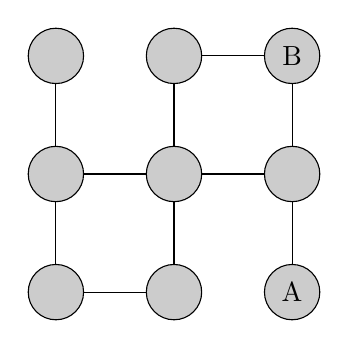
\begin{tikzpicture}[darkstyle/.style={circle,draw,fill=gray!40,minimum size=20}]
  \foreach \x in {0,...,2}
    \foreach \y in {0,...,2} 
       {\node [darkstyle]  (\x\y) at (1.5*\x,1.5*\y) {\ifthenelse{\x=2 \AND \y=0}{A}{\ifthenelse{\x=2\AND\y=2}{B}{}}};} 

       \draw (00)--(01);
       \draw (01)--(02);

       \draw (10)--(11);
       \draw (11)--(12);

       \draw (10)--(11);
       \draw (11)--(21);

       \draw (20)--(21);
       \draw (11)--(21);

       \draw (21)--(22);
       \draw (01)--(11);
       \draw (00)--(10);
       \draw (12)--(22);


\end{tikzpicture}
\end{center}
The robot moves in exactly one direction each turn (and must move). The robot's goal is to maximize its score in the game after $T$ steps. The
score is defined in the following way:
%
\begin{itemize}
  \item If the robot attempts to move off the grid, then the robot loses a point (-1) and stays where it is.
  \item If the robot moves onto node A, it receives 10 points, and if it moves onto node B, it receives 5 points. Otherwise, it receives 0 points.
\end{itemize}

  \begin{enumerate}
    \item Model this as a Markov decision process: define the states $S$, actions $A$, reward function $r:S\times A\mapsto \mathbb{R}$, and transition model $p(s'\given s, a)$ for $s', s\in S$ and $a\in A$.
%
%, \mathcal{A}, \mathcal{R}, \mathcal{P}$) are in this problem.
    \item Consider a \emph{random policy} $\pi$, where
in each state the robot moves uniformly at randomly in any of its available directions (including off the board). 
      For every position on the grid calculate the
value function, $V^\pi_t: S\mapsto 
\mathbb{R}$, under this policy, for $t=2, 1$ steps left
to go. You can find LaTeX code for the tables in the solution template. Note that you should have 2 tables, one for each time horizon. 
%
    \item Now assume that the robot plays an \emph{optimal policy}
      $\pi^\ast_t$ (for $t$ time steps to go). Find the optimal policy in the case of a finite time horizon of $t = 1, 2$ and give the corresponding 
MDP value functions $V^\ast_t: S\mapsto 
\mathbb{R}$, under this
optimal policy. You can indicate the optimal policy for each time horizon on the corresponding $V^\ast_t$ table via arrows or words in the direction that the robot should move from that state. 
    \item Now consider the situation where the robot does not have
      complete control over its movement. In particular, 
when it chooses a direction, there is a 80\% chance that it will go in
      that direction, and a 10\% chance it will go in the two adjacent
      (90$^\circ$ left or 90$^\circ$ right) 
directions. Explain how this changes the elements $S$, $A$, $r$, and $p(s' \given s,a)$ of the MDP model. 
Assume the robot uses the same
 policy $\pi^\ast_t$ from the previous question (now possibly
      non-optimal), and write this as $\pi_t$, and tie-break in favor of N, then E, then S then W.
Give the corresponding 
MDP value functions $V^\pi_t: S\mapsto 
\mathbb{R}$, for this policy in this partial control world, for $t=2, 1$ steps left
to go. Is the policy still optimal?
  \end{enumerate}
\end{problem}
%\subsection*{Solution}

%  Table starter code
%  \begin{center}
%    \begin{tabular}{c|c}
%      $s$ & $V^\pi_1(s)$ \\ \hline
%      State & 0
%    \end{tabular}
%  \end{center}

\newpage

\section*{The Viterbi Algorithm [15 pts]}

{\bf Problem 4}
\medskip

In this problem, you will use Hidden Markov Models to reconstruct
state sequences in data after learning from complete-data labeled
sequences.

We consider a simple robot that moves across colored squares. At each
time step, the robot attempts to move up, down, left or right, where
the choice of direction is made at random.  If the robot attempts to
move onto a black square, or to leave the confines of its world, its
action has no effect and it does not move at all.  The robot can only
sense the color of the square it occupies.  Moreover, its sensors are
only 90\% accurate, meaning that 10\% of the time, it perceives a
random color rather than the true color of the currently occupied
square.  The robot begins each walk in a randomly chosen colored
square.


\begin{center}
  \includegraphics[width=1.5in]{robot_maze.png}
\end{center}

In this problem, state refers to the location of the robot in the
world in $x:y$ coordinates, and output refers to a perceived color
({\tt r}, {\tt g}, {\tt b} or {\tt y}). Thus, a typical random walk
looks like this:



\begin{verbatim}
3:3 r
3:3 r
3:4 y
2:4 b
3:4 y
3:3 r
2:3 b
\end{verbatim}

Here, the robot begins in square 3:3 perceiving red, attempts to make
an illegal move (to the right), so stays in 3:3, still perceiving red.
On the next step, the robot moves up to 3:4 perceiving yellow, then
left to 2:4 perceiving blue (erroneously), and so on. By learning
on this data, you will build an HMM model of the world.
Then, given only sensor observations (i.e., a sequence of colors), the
Viterbi code will re-construct an estimate of the actual path taken by
the robot through its world.

The data for this problem is in {\tt robot\_no\_momentum.data}, a file
containing 200 training sequences (random walks) and 200 test
sequences, each sequence consisting of 200 steps. We are also
providing data on a variant of this problem in which the robot's
actions have ``momentum'' meaning that, at each time step, with 85\%
probability, the robot continues to try to move in the direction of the last
move.  So, if the robot moved (successfully) to the left on the last
move, then with 85\% probability, it will again attempt to move left.
If the robot's last action was unsuccessful, then the robot reverts to
choosing an action at random.  Data for this problem is in {\tt
  robot\_with\_momentum.data}.

\noindent { [Acknowledgment: thanks Rob Schapire for allowing us to
use his robot dataset for this homework.]}

\pagebreak

% \begin{problem}
% ~


% \vspace{-0.75cm}

\begin{enumerate}

\item  \textbf{Learning a HMM model from labeled data.}

Recall that a Hidden Markov Model is specified by three sets of
probabilities: the initial probabilities of starting in each state ($\btheta$ ),
the probabilities of transitioning between each pair of hidden states ($\boldT$),
and the probabilities of each output in each state ($\bpi$).  Your job will be
to compute estimates of these probabilities from data.  We are
providing you with training data consisting of one or more sequences
of state-observation pairs, i.e., sequences of the form
\[\bolds_1, \boldx_1, \bolds_2, \boldx_2, \cdots, \bolds_n, \boldx_n\]

For this problem, we will assume that the states are observed while
training (complete data assumption).  Given these sequences, you need
to estimate the probabilities that define the HMM. 

Note: We will make one modification to complete-data
maximum-likelihood estimation described in Lecture 17 for all
parameters. Instead of estimating using MLE we will use a method known
as \emph{Laplace smoothing}, where an additional pseudo-count is added
to each class. For instance, instead of using $\hat{\theta}_k =
\frac{N_{1,k}}{N}$ for the estimate of the starting state, we will use
$\hat{\theta}_k = \frac{N_{1,k}+ 1}{N + c}$, where there are $c$
states in total. This ensures that no sequences have zero probability.
(This method can also be shown to correspond to a Bayesian approach,
with the pseudocount arising from a Dirichlet prior on the Categorical
distribution. )

\textbf{Task:} First, familiarize yourself with the provided code. Your first programming
task is to fill in the {\tt learn\_from\_labeled\_data} function in
{\tt hmm.py}  

{\bf Testing:} Check the code passes {\tt test\_learn\_from\_labeled\_data} in {\tt
  test\_hmm.py}.




\item \textbf{Computing the most likely sequence of hidden states (short sequences).}

  Now that we have learned a model, we can use the Viterbi algorithm
  to compute the most likely sequence of hidden states given a
  sequence of observations. 
  
  The second part of the dataset consists of test sequences of
  state-observation pairs.  The Viterbi code accepts as input just the
  observation part of each of these sequences, and from this, will compute
  the most likely sequence of states to produce such an observation
  sequence. The state part of these sequences is provided so that you
  can compare the estimated state sequences generated by the algorithm
  to the actual state sequences.  Note that these two sequences will
  not necessarily be identical, even for a correct implementation of
  the Viterbi algorithm.

  \textbf{Task:}  Implement the Viterbi algorithm to fill in the {\tt most\_likely\_states} function in
{\tt hmm.py}  

  \textbf{Testing:} 
  Confirm that your code 
  passes {\tt test\_viterbi\_simple\_sequence} in  {\tt test\_hmm.py}.

\item \textbf{Computing the most likely sequence of hidden states (long sequences).}
  
  In practice, the method described in the lecture notes will not
  actually work for longer sequences. This issue arises due to
  numerical underflow to to the repeated multiplication of
  probabilities. We can avoid this problem, by instead computing the
  most likely sequence in log-space, i.e.
  \[\arg\max_{\bolds_{1}\ldots \bolds_{n}}\log p(\bolds_1, \ldots
  \bolds_n, \boldx_1, \ldots, \boldx_n).\]
  Mathematically, this is the same, but will avoid the numerical
  issues.
 
 

 \textbf{Task:} Change the code in {\tt most\_likely\_states} to use logs of the probabilities
instead of the probabilities directly.  

\textbf{Testing:} Check the code now also passes {\tt test\_viterbi\_long\_sequence} in  {\tt test\_hmm.py}.

\item   \textbf{Experimenting with data.}

Finally run {\tt viterbi.py} on the two robot data files, {\tt robot\_no\_momentum.data} and \\{\tt robot\_with\_momentum.data} and examine the results,
  exploring how, why and when it works. To get the the breakdown of the error, set \texttt{debug=True} in the code. Sample command-line prompt: 
  \begin{lstlisting}[language=bash]
  $ python viterbi.py robot_small.data -v
\end{lstlisting}
  You should write up {\em
    briefly} what you found.
  Your write-up should include any observations you  have made
  about how well HMMs work on this problem and why.  Your observations
  should be quantitative (for instance, the number of errors was $x$) as well
  as anecdotal (situations where the approach failed).                                                                                                                                                                     
                                                                                                                                                                                 
  Although this write-up is quite open ended, {\bf you should be sure to                                                                                                           
    discuss the following}:
%
\begin{itemize}
\item  What probabilistic assumptions are we making                                                                                                           
  about the nature of the data in using a hidden Markov model?
\item   How well                                                                                                           
  do those assumptions match the actual process generating the data?                                                              \item                                                 
  And to what extent was or was not performance hurt by making such                                                                                                                
  realistic or unrealistic assumptions?  
\end{itemize}

\end{enumerate}

%\end{problem}
%\subsection*{Solution}

\end{document}
